\documentclass[a4paper, 7px]{article}
\usepackage{amsmath}
\usepackage{graphicx}
\usepackage{hyperref}
\usepackage[a4paper,landscape, margin=2mm]{geometry}
\usepackage{tikz}
\usetikzlibrary{positioning}

\title{Two Wheel (name TBD)}
\author{Lorenzo Boglione}

\makeindex

\begin{document}
\maketitle
\newpage


\section{Structure}
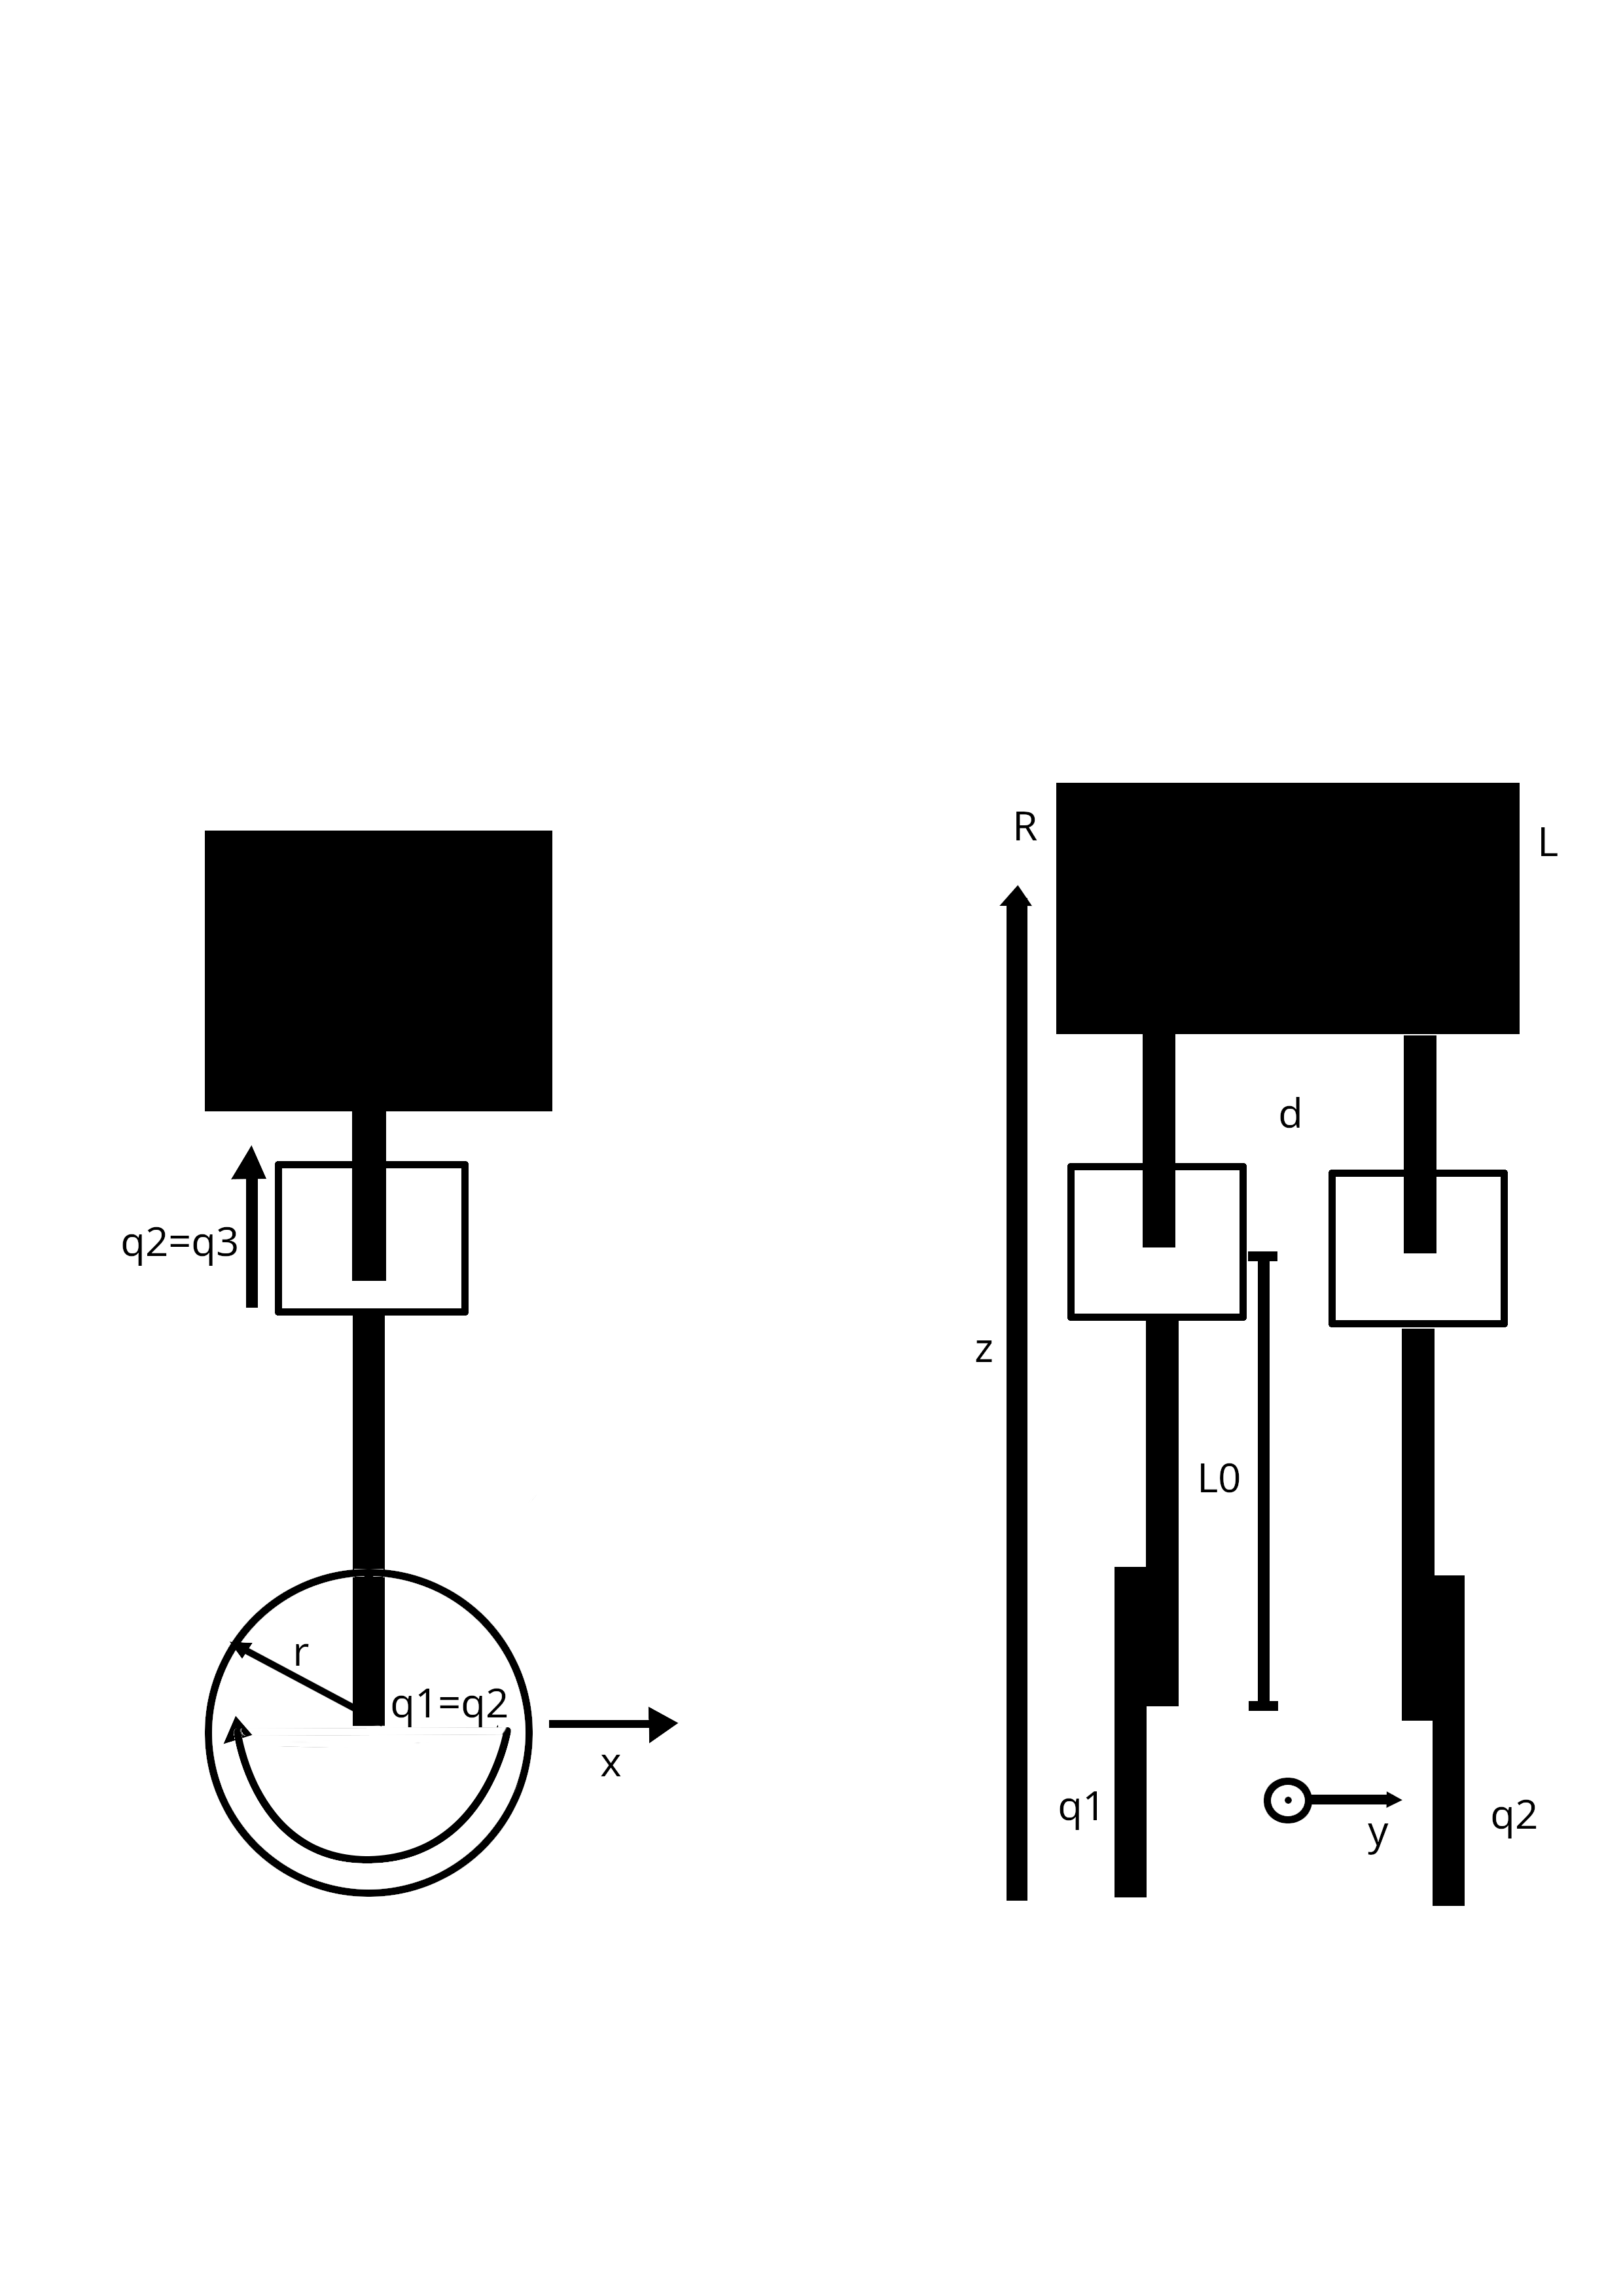
\includegraphics[height=100mm]{Schematic_png}
\section{Kinematic}

\subsection{Variables}
Coordinates:
$$p = 
\begin{bmatrix}
	x\\ 
	y\\
	z\\ 
	\theta_x\\
	\theta_z\\ 
	
\end{bmatrix}
$$
Joint Variables:
$$q = 
\begin{bmatrix}
	\theta_R\\
	\theta_L\\
	d_L\\
	d_R\\
\end{bmatrix} =  
\begin{bmatrix}
	q_1\\ 
	q_2\\ 
	q_3\\
	q_4\\
\end{bmatrix}$$

Simplified system(q3=q4=const)

Generalized Coordinates:
$$u = 
\begin{bmatrix}
	d\\
	\theta_x\\
	\theta_z\\ 	
\end{bmatrix}$$

Joint Variables:
$$q = 
\begin{bmatrix}
	\theta_R\\
	\theta_L\\
\end{bmatrix} =  
\begin{bmatrix}
	q_1\\ 
	q_2\\ 
\end{bmatrix}$$
\subsection{Constraint Definition}
Diff drive constrain:
$$ \frac{dy}{dx}=tan(\theta_z)$$
$$ 
\begin{bmatrix} 
	sin(\theta_z)\\
 	cos(\theta_z)\\ 
 	0\\ 
 	0\\ 
 	0\\ 
\end{bmatrix} 
 * p = 0$$
We obtain the following G matrix
$$G = 
\begin{bmatrix}
c_{\theta_z} & 0 & 0 & 0\\
s_{\theta_z} & 0 & 0 & 0\\
0 & 1 & 0 & 0\\
0 & 0 & 1 & 0\\
0 & 0 & 0 & 1\\
\end{bmatrix}$$
$$\dot p = G \dot u = G 
\begin{bmatrix}
	v\\
	v_z\\
	\omega_x\\
	\omega_z\\
	
\end{bmatrix}$$
We can find a correlation between the u vector and q as
$$ \dot u = T \dot q$$
$$ T = 
\begin{bmatrix}
	\frac{r}{2} & \frac{r}{2} & 0 & 0\\
	0 & 0 & \frac{1}{2} & \frac{1}{2}\\
	0 & 0 & \frac{1}{d} & -\frac{1}{d}\\	
	-\frac{r}{\sqrt{d^2 + (d_R - d_L)^2}} & 				\frac{r}{\sqrt{d^2 + (d_R - d_L)^2}} & 0 & 0\\
	
\end{bmatrix}$$
$$G_q = G*T =  
\begin{bmatrix}
	r\frac{c_{\theta_z}}{2} & r\frac{c_{\theta_z}}{2} & 0 & 0\\
	r\frac{s_{\theta_z}}{2} & r\frac{s_{\theta_z}}{2} & 0 & 0\\
	0 & 0 & \frac{1}{2} & \frac{1}{2}\\
	0 & 0 & \frac{1}{d} & -\frac{1}{d}\\
	-\frac{r}{\sqrt{d^2 + (d_R - d_L)^2}} & 				\frac{r}{\sqrt{d^2 + (d_R - d_L)^2}} & 0 & 0\\
	 
\end{bmatrix}$$

$$\dot p = G_q \dot q$$


For the simplified system we already have the minimum number of coordinates so we only need to convert the generalized coordinates into physically meaning coordinate (joint variable)

$$ \dot q = T * \dot u$$
$$ \omega_R = \frac{v + \omega_z*\frac{d}{2}}{r} - \omega_y$$ 
$$ \omega_L = \frac{v - \omega_z*\frac{d}{2}}{r} - \omega_y$$
$$ T = 
\begin{bmatrix}
	\frac{1}{r} & -1 & \frac{d}{2 \, r}\\
	\frac{1}{r} & -1 & -\frac{d}{2 \, r}\\
\end{bmatrix}
$$
\newpage
\section{Dynamic}
For the dynamic we need to consider a third variable $\theta_y$

$$p = 
\begin{bmatrix}
	x\\
	y\\
	z\\
	\theta_x\\
	\theta_y\\
	\theta_z\\
\end{bmatrix}$$

And since no joint directly controls the orientation we can expand $G_q$ as follows:
$$G_q =  
\begin{bmatrix}
	r\frac{c_{\theta_z}}{2} & r\frac{c_{\theta_z}}{2} & 0 & 0\\
	r\frac{s_{\theta_z}}{2} & r\frac{s_{\theta_z}}{2} & 0 & 0\\
	0 & 0 & \frac{1}{2} & \frac{1}{2}\\
	0 & 0 & \frac{1}{d} & -\frac{1}{d}\\
	0 & 0 & 0 & 0\\
	-\frac{r}{\sqrt{d^2 + (d_R - d_L)^2}} & 				\frac{r}{\sqrt{d^2 + (d_R - d_L)^2}} & 0 & 0\\
\end{bmatrix}$$	

\subsection{Kinetic energy}
Let's take into consideratio one body at a time ignoring for the moment the motor's contribution: 
\begin{enumerate}
	\item Right Wheel
	\item Left Wheel
	\item Right Leg
	\item Left Leg
	\item Body
\end{enumerate}


\begin{huge}
	Change everything as function of u
\end{huge} \\


Express everything within respect to $\dot u = \begin{bmatrix}
v\\ v_z\\ \omega_x \\ \omega_y \\ \omega_z
\end{bmatrix} $

$$
K_1 =
\begin{cases}
	K_1 = \frac{1}{2} m_W v_{W_R}^2 + \frac{1}{2}\omega_{W_R}^T \Gamma_W \omega_{W_R}\\
	v_{W_R} = v + \omega_z \frac{\sqrt{d^2 + (d \, tan(\theta_x))^2}}{2}\\
	\omega_{W_R} = 
		\begin{bmatrix}
			\dot \theta_x\\
			\dot q1 + \dot \theta_y\\
			\dot \theta_z\\
		\end{bmatrix}
		=
		\begin{bmatrix}
			\omega_x\\
			\frac{v_{W_R}}{r} + \omega_y\\
			\omega_z\\
		\end{bmatrix}
		\\
		Gamma_{W_R} = ...
\end{cases}
$$

$$
K_2 =
\begin{cases}
	K_2 = \frac{1}{2} m_W v_{W_L}^2 + \frac{1}{2}\omega_{W_L}^T \Gamma_W \omega_{W_L}\\
	v_{W_L} = v  - \omega_z \frac{\sqrt{d^2 + (d \, tan(\theta_x))^2}}{2}\\
	\omega_{W_L} = 
		\begin{bmatrix}
			\omega_x\\
			\dot q2 + \omega_y\\
			\omega_z\\
		\end{bmatrix}=
		\begin{bmatrix}
			\omega_x\\
			\frac{v_{W_L}}{r} + \omega_y\\
			\omega_z\\
		\end{bmatrix}
\end{cases}
$$

$$
K_3 =
\begin{cases}
	K_3 = \frac{1}{2} m_L v_{L_R}^2 + \frac{1}{2}\omega_{L_R}^T \Gamma_L \omega_{L_R}\\
	v_{L_R} = v + \omega_z \frac{\sqrt{d^2 + (d \, tan(\theta_x))^2}}{2}\\
	\omega_{L_R} = 
		\begin{bmatrix}
			\omega_x\\
			\omega_y\\
			\omega_z\\
		\end{bmatrix}
\end{cases}
$$

$$
K_4 =
\begin{cases}
	K_4 = \frac{1}{2} m_L v_{L_L}^2 + \frac{1}{2}\omega_{L_L}^T \Gamma_L \omega_{L_L}\\
	v_{L_L} = v - \omega_z \frac{\sqrt{d^2 + (d \, tan(\theta_x))^2}}{2}\\
	\omega_{L_L} = 
		\begin{bmatrix}
			\omega_x\\
			\omega_y\\
			\omega_z\\
		\end{bmatrix}
\end{cases}
$$

$$K_5 = 
\begin{cases}
	K_4 = \frac{1}{2} m_B v_B^2 + \frac{1}{2}*\omega_B^T \Gamma_B \omega_B\\
	v_B = v + p_B X \omega_B\\
	\omega_B = 
		\begin{bmatrix}
			\omega_x\\
			\omega_y\\
			\omega_z\\
		\end{bmatrix}\\
		p_B = \begin{bmatrix}
		0\\
		0\\
		z\\
		\end{bmatrix}
		
\end{cases}
$$

\subsection{Potential energy}
With the same assumptio made before we can notice that we have only gravitational contribution.
We can consider the 0 plane at the wheel height and 

$$
U=
\begin{cases}
	U_1 = 0\\
	U_2 = 0\\
	U_3 = \frac{L_0  sin(\theta_x)sin(\theta_y)}{2}m_L\,g\\
	U_4 = \frac{L_0sin(\theta_x)sin(\theta_y)}{2}m_L\,g\\
	U_5 = zsin(\theta_x)sin(\theta_y)\,m_B\,g\\
\end{cases}
=
g(u)
$$

\subsection{External forces}

As first approximation we can neglect the dissipative forces as frictions.
The forces taken into account are the reaction force and the gravity force of the body mass.

$$f_r : 
\frac{\delta W_{f_r}}{\delta u} = 0
$$

$$f_g :
\begin{cases}
	
	\frac{\delta W_{f_g}}{\delta d} = 0\\
	
	\frac{\delta W_{f_g}}{\delta z} = 
\end{cases}$$
	
 


\subsection{Lagrange Equations}
Knowing both kinetic and potential energy we can start computing the left part of the lagrange equations

$$\frac{d}{dt}\bigg (\frac{\delta L}{\delta \dot u} \bigg) - \bigg( \frac{\delta L}{\delta u} \bigg )$$

$$\frac{\delta L}{\delta \dot u} = 
\begin{bmatrix}

	2 ( m_L + m_W + \frac{\Gamma_W}{r^2})v + \frac{ m_B ( 2 v - 2 \omega_y z)}{4 \sqrt{\omega_x^2 z^2 +  \omega_y^2 z^2 - 2 \omega_y v\, z + v^2+ v_z^2}} + \frac{2 \Gamma_W \omega_y}{r}\\
	
	\frac{m_B}{2 \sqrt{\omega_x^2 z^2 + \omega_y^2 z^2 - 2 \omega_y v \, z + v^2 + v_z^2}}v_z\\
	
	2(\frac{\Gamma_B}{2} + \Gamma_L + \Gamma_W)\omega_x + \frac{m_B}{2\sqrt{\omega_x^2 z^2 + \omega_y^2 z^2 - 2 \omega_y v \, z + v^2 + v_z^2}}\omega_x z^2\\	
	
	2(\frac{\Gamma_B}{2} + \Gamma_L + \Gamma_W) \omega_y + \frac{2 \Gamma_W}{r} v - \frac{m_B z (v - \omega_y z)}{2\sqrt{\omega_x^2 z^2 + \omega_y^2 z^2 - 2 \omega_y v \, z + v^2 + v_z^2}}\\

	2 \omega_z (\frac{\Gamma_B}{2} + \Gamma_L + \Gamma_W + \frac{d \, m_L (tan(\theta_x)^2 + d)}{4} + \frac{d \, m_W (tan(\theta_x)^2 + d)}{4} + \frac{\Gamma_W | d(tan(\theta_x)^2 + d) |}{4 r^2})
	
\end{bmatrix}
$$
We can make some assumpion, first the 

$$
\frac{d}{dt} \bigg( \frac{\delta L}{\delta \dot u} \bigg)= 
\begin{bmatrix}
	

 

\end{bmatrix}
$$


\section{Simplified Dynamic}
\subsection{Kinetic Energy}
$$
K1 = 
\begin{cases}
	K1 = \frac{1}{2} m_W v_1^2 + 1/2 \omega_1^T \Gamma_W \omega_1 \\
	v_1 = v + \frac{d}{2} \omega_z\\
	\omega_1 =
	\begin{bmatrix}
		0\\
		\frac{v1}{r}\\
		\omega_z\\
	\end{bmatrix}
\end{cases}
$$

$$
K1 = 
\begin{cases}
	K2 = \frac{1}{2} m_W v_2^2 + 1/2 \omega_2^T \Gamma_W \omega_2 \\
	v_2 = v - \frac{d}{2} \omega_z\\
	\omega_2 =
	\begin{bmatrix}
		0\\
		\frac{v2}{r}\\
		\omega_z\\
	\end{bmatrix}
\end{cases}
$$

$$
K3 = 
\begin{cases}
	K3 = \frac{1}{2} m_B v_3^2 + 1/2 \omega_3^T \Gamma_B \omega_3 \\
	v_3 = v + l \omega_y\\
	\omega_3 =
	\begin{bmatrix}
		0\\
		\omega_y\\
		\omega_z\\
	\end{bmatrix}
\end{cases}
$$
\subsection{Potential Energy}
$$ U = l \, cos(\theta_y) \, g$$

\subsection{Lagrange equation}
$$L = \frac{\Gamma _{b,\mathrm{yy}}\,{\left|\frac{\partial }{\partial t} \theta _{y}\left(t\right)\right|}^2}{2}+\frac{\Gamma _{b,\mathrm{zz}}\,{\left|\frac{\partial }{\partial t} \theta _{z}\left(t\right)\right|}^2}{2}+\Gamma _{w,\mathrm{zz}}\,{\left|\frac{\partial }{\partial t} \theta _{z}\left(t\right)\right|}^2+\frac{m_{w}\,{\left|-\frac{d\,\frac{\partial }{\partial t} \theta _{z}\left(t\right)}{2}+\frac{\partial }{\partial t} p\left(t\right)\right|}^2}{2}+\frac{m_{w}\,{\left|\frac{d\,\frac{\partial }{\partial t} \theta _{z}\left(t\right)}{2}+\frac{\partial }{\partial t} p\left(t\right)\right|}^2}{2}+\frac{m_{w}\,{\left|l\,\frac{\partial }{\partial t} \theta _{y}\left(t\right)+\frac{\partial }{\partial t} p\left(t\right)\right|}^2}{2}-g\,l\,\cos\left(\theta _{y}\left(t\right)\right)+\frac{\Gamma _{w,\mathrm{yy}}\,{\left|-\frac{d\,\frac{\partial }{\partial t} \theta _{z}\left(t\right)}{2}+\frac{\partial }{\partial t} p\left(t\right)\right|}^2}{r^2\,2}+\frac{\Gamma _{w,\mathrm{yy}}\,{\left|\frac{d\,\frac{\partial }{\partial t} \theta _{z}\left(t\right)}{2}+\frac{\partial }{\partial t} p\left(t\right)\right|}^2}{r^2\,2}$$




$$B \ddot{u} + g(u) = \gamma$$

$$B = 
\begin{bmatrix}
	\Gamma _{w,\mathrm{yy}}+3\,m_{w} & l\,m_{w} & 0\\
	l\,m_{w} & m_{w}\,l^2+\Gamma _{b,\mathrm{yy}} & 0\\
	0 & 0 & \Gamma _{b,\mathrm{zz}}+2\,\Gamma _{w,\mathrm{zz}}+\frac{d^2\,m_{w}}{2}+\frac{\Gamma _{w,\mathrm{yy}}\,d^2}{2\,r^2} \end{bmatrix}
$$
$$g(u) = 
\begin{bmatrix}
	0\\
	-g \, l \, \sin{\theta_y}\\
	0
\end{bmatrix}
$$
$$\gamma = \, forces \, on \, generalized \, coordinates = T^T \,  \tau$$
$$\tau = (T^+)^T \, \gamma$$
%\section{Controller}
%\begin{tikzpicture}
%	\node [draw, circle, minimum size = 0.6cm] (sum_P) at (0,0) {};
%	\node [draw, circle, minimum size = 0.6cm, below and right  of %sum_P]  (sum_I) {};
%\end{tikzpicture}
%\section{Simplified Controller}


\section{ROS}

\subsection{Simulation}

The simulation is performed with Gazebo since it provides an easy interface with ROS.
The robot model along with the sensor's definition is done via an urdf file.

\subsubsection{Controller}
The interface between Gazebo and ROS is enstablished via the \href{https://github.com/ros-controls/ros2_control}{ros controls} 
and \href{https://github.com/ros-controls/gazebo_ros2_control}{gazebo ros2 control}.

The controller allows 3 sets of feedback:
\begin{enumerate}
	\item position feedback
	\item velocity feedback
	\item position and velocity feedback
\end{enumerate}

in the future might be added a trajectory following controller that will perform a position velocity and acceleration feedback

\end{document}